\documentclass[a4,10pt]{article} \usepackage[pdftex]{graphicx}
\usepackage{setspace}
%\usepackage{lineno}
\usepackage{color}
\usepackage{hyperref}
\hypersetup{
    colorlinks,%
    citecolor=black,%
    filecolor=black,%
    linkcolor=black,%
    urlcolor=blue
}
\definecolor{PiranaOrange}{rgb}{0.9,0.4,0.1}
\definecolor{Blue}{rgb}{0.0,0.0,0.7}
\definecolor{Red}{rgb}{0.7,0.0,0.0}
\definecolor{Grey}{rgb}{0.2,0.2,0.2}
\definecolor{grey2}{rgb}{.92, .92, .92}

\pdfinfo{
   /Author (Ron Keizer, Coen van Hasselt, Pirana Software & Consulting BV)
   /Title  (Pirana Quick Guide)
}



\bibliographystyle{unsrt}%Choose a bibliograhpic style}
%\usepackage{utopia} %\usepackage{charter} %\usepackage{palatino}
%\usepackage{bookman} %\usepackage{newcent} %\usepackage{times}
%\usepackage[options]{natbib} \sloppy
\renewcommand{\familydefault}{\sfdefault} 
\renewcommand{\emph}[1]{\textbf{\textcolor{Grey}{#1}}} 
\oddsidemargin 1cm
\textwidth 14cm
\textheight 20cm

\begin{document}

{\centering
  \vspace{-100pt}
  \textbf{
    \textcolor{PiranaOrange}{\Large Pirana}
  }\\
  \vspace{5pt} \scriptsize \textcolor{Grey}{The flexible modeling
    environment for NONMEM} \\ \normalsize
  \vspace{12pt}
  \hspace{5pt}
\includegraphics[scale=0.14]{images/pirana_logo.jpg}\\
  \vspace{18pt}

  {\large \emph{Quick Guide: Diagnostic graphics in Pirana using the
      integrated R-scripts library (without Xpose)} \vspace{10pt}
    \\ Version 1.1 }

}
\vspace{25pt}

\begin{center}
   {\colorbox{grey2}{
         \begin{minipage}[t]{0.9\textwidth}
\subsubsection*{Scope}
This Pirana Quick Guide explains how to use Pirana to generate and
modify diagnostic graphs using the integrated R scripts library.
          \end{minipage}
      }
   }
\end{center}

\vspace{10pt}

Pirana has an integrated library of R scripts which can be used to
generate diagnostic plots based on model output files. The library of
R scripts can also be easily edited or extended with new scripts.

\subsubsection*{Creating diagnostic plots}
\begin{itemize}
\item Select the model for which you want to create plots.
\item In the right panel under Scripts, select the desired script.
\item Via the context menu, select run script. 
  clicking the right mouse button, and then selecting 'Run script',
  and subsequently selecting the plot you want to create (Figure \ref{fig:Fig1}).
\item The plot will be created and openened automatically (Figure \ref{fig:Fig2}).
 
\end{itemize}


\begin{figure}[hctb] \centering
    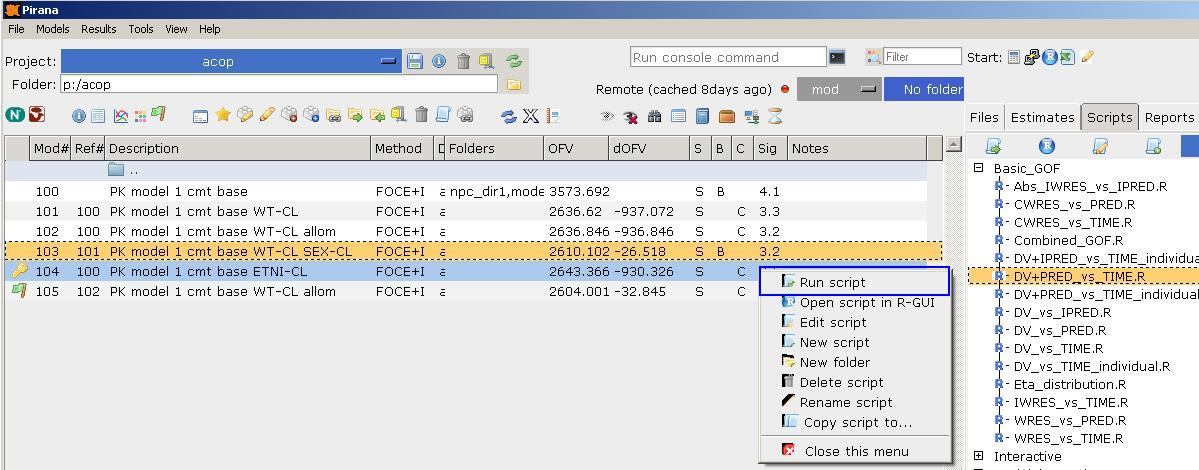
\includegraphics[scale=.3]{images/graphs_1.jpg}
    \caption{Running a script on a model run\label{fig:Fig1}}
\end{figure}

\begin{figure}[h] \centering
    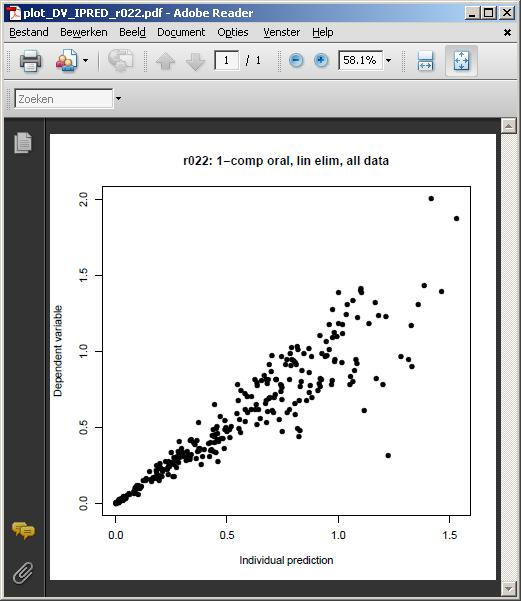
\includegraphics[scale=.45]{images/graphs_3.jpg}
    \caption{Diagnostic plot created\label{fig:Fig2}}
\end{figure}


\subsubsection*{Troubleshooting problems with plot creation}
\begin{itemize}
\item If an error occurs, the R output will be displayed, which can be
used to diagnose the error (Figure \ref{fig:Fig3}). 
\item Most frequently this is due to a variable missing in the output table 
files (e.g. column IPRED not available in output table).
\item The expected input variables for each script are depicted at the bottom of 
the right panel. 
\end{itemize}

\begin{figure}[hctb] \centering
    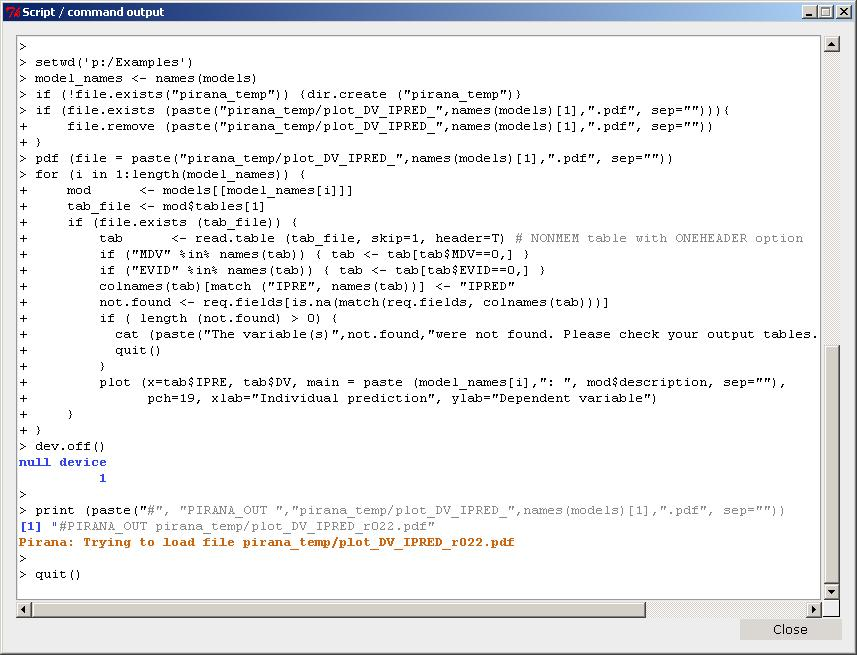
\includegraphics[scale=.45]{images/graphs_2.jpg}
    \caption{Output of the script\label{fig:Fig3}}
\end{figure}


\subsubsection*{Customizing diagnostic plots}
\begin{itemize}
\item Instead of running the script through Run Script (above), the
  script may also be outputted to the R GUI ("Output script to R GUI")
  (Figure \ref{fig:Fig4}). Now, you can easily tweak the plot, and save it in the
  format you like. 
\item Afrter sending the script to R GUI, it will be opened there,
  where it may be further modified. Next, the script can be executed
  and the plot will be created within the R GUI (Figure 5).
\end{itemize}

\begin{figure}[h] \centering
    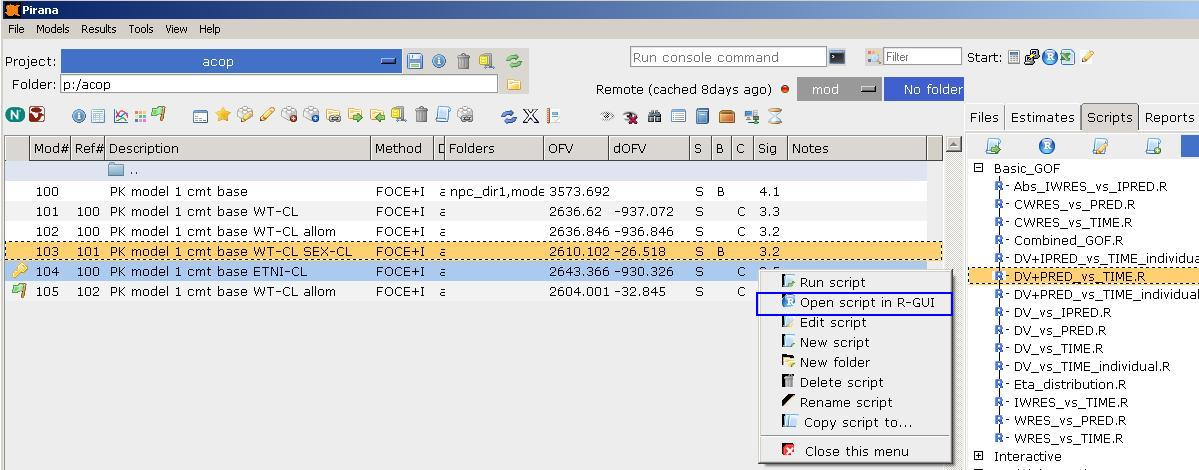
\includegraphics[scale=.3]{images/graphs_4.jpg}
    \caption{Output of a script to the R GUI for further customization\label{fig:Fig4}}
\end{figure}


\subsubsection*{Editing and creating scripts}
\begin{itemize}
\item When one whishes to permanently make changes to the scripts
  library, this can be done using the option "Edit script" in the right panel context menu.
  (Figure \ref{fig:Fig6}).
\item Any changes made to the script will be saved permanently. You
  can choose to make changes in the script that are originally
  supplied with Pirana, or have them in your own user library.
\item Script files are located either in the user folder
  (e.g. C:$\backslash$Documents and
  Settings$\backslash$Username
$\backslash$.pirana$\backslash$scripts), or in the
  main Pirana folder (e.g. C:$\backslash$Program
  Files$\backslash$Pirana). The organization of scripts in sub-menus
  is according to the folder structure in these scripts folders
  (Figure \ref{fig:Fig7}), and can be adjusted accordingly.
\item Note that when you install a new version of Pirana over the old
  one, any R script you have in the Pirana folder will be overwritten
  with the one supplied by the new version of Pirana (if you haven't
  given the R-script another name).
\item Through the menu 'Scripts' $\rightarrow$ 'New scripts', it is
  also possible to define new scripts. Please note that at current,
  you will have to restart Pirana for the script to show up in the
  interface.
\end{itemize}

\begin{figure}[h] \centering
    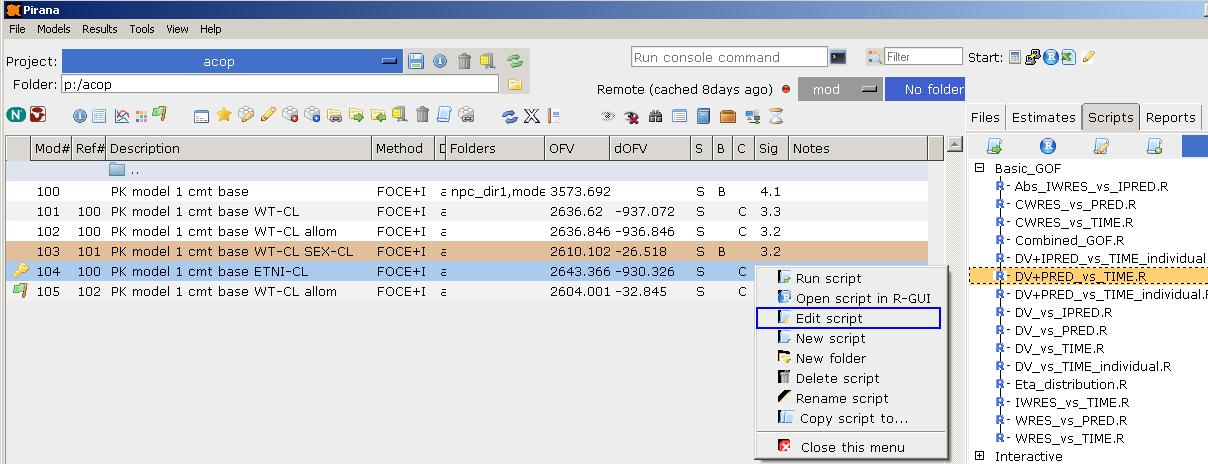
\includegraphics[scale=.3]{images/graphs_6.jpg}
    \caption{Editing templates for scripts\label{fig:Fig6}}
\end{figure}

\begin{figure}[h] \centering
    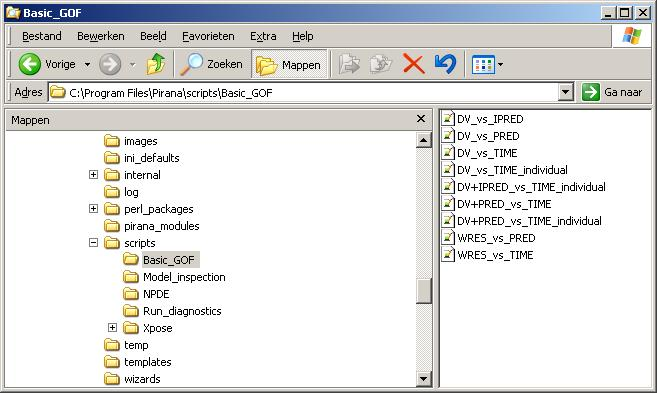
\includegraphics[scale=.5]{images/graphs_7.jpg}
    \caption{Script files present in the scripts sub-folder of Pirana\label{fig:Fig7}}
\end{figure}



\end{document}
